%7
\section{Paketdetails}

%7.1 Paket Robot
\subsection{Paket \textit{Robot}}
	\begin{figure}[H]
	\centering
	\includegraphics[width=0.6\textwidth]{../images/Paketdetails.png}
	\caption{\textcolor{blue}{HIER KOMMT DAS ROBOT - PAKETDIAGRMAM HIN}}
	\label{Paketdetails}
	\end{figure}
	Im folgenden beschreiben wir die wichtigen Klassen des Pakets \textit{Robot} 
	und ihre zugehörigen wichtigen Methoden, sowie ihre Interaktion zwischeneinander. 


	%7.1.1 RobotController
	\subsubsection{Beschreibung der Klasse \textit{RobotController}}
		\begin{figure}[H]
		\centering
		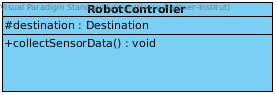
\includegraphics[width=0.6\textwidth]{../images/Iteration0_Entwurf_7-1-1_Klasse_RobotController}
		\caption{\textcolor{blue}{Durch eigene Diagramme ersetzen}}
		\label{BeschreibungKlasse1}
		\end{figure}
		
		%#destination : Destination
		Die Klasse \textit{RobotController} ist die Hauptklasse des \textit{Robots}, 
		da sie den aktuellen Zustand des \textit{Robots} enthält.
		So hat diese Klasse die Möglichkeit höchstens eine \textit{Destination} zu speichern. 
		Diese \textit{Destination} kann ein vom \textit{Server} zugeteiltes Ziel sein, 
		der dem \textit{Robot} zugehörige \textit{Charger}, oder gerade kein Ziel, 
		also \textit{null} sein. Nur wenn der \textit{Robot} gerade keine \textit{Destination} 
		gespeichert hat, kann er neue Aufträge vom \textit{Server} annehmen.

			%7.1.1.1 #collectSensorData():void
			\paragraph{Beschreibung der Methode \textit{collectSensorData}}
			Die Methode \textit{collectSensorData} wird von der Methode \textit{recieveMessage} 
			aus der Klasse \textit{RobotCommunication} aufgerufen, wenn eine Neue \textit{Message} 
			vom Server eingegangen ist, welche den \textit{Robot} dazu auffordert, Informationen 
			über seinen Zustand zu senden. Der \textit{Robot} fragt dann seine Hardwareschnittstelle 
			nach seiner Position und seinem Akkustand an, und verfasst eine neue \textit{Message} 
			die diese Informationen, sowie seinen Aktuellen Zustand bzw. seine aktuelle \textit{Destination} enthalten.

	%7.1.2 DrivingSystem
	\subsubsection{Beschreibung der Klasse \textit{DrivingSystem}}
		\begin{figure}[H]
		\centering
		\includegraphics[width=0.6\textwidth]{../images/Iteration0_Entwurf_7-1-2_Klasse_DrivingSystem}
		\caption{\textcolor{blue}{Durch eigene Diagramme ersetzen}}
		\label{BeschreibungKlasse1}
		\end{figure}
		
		%#currentSpeed:float
		Diese Klasse beschreibt den aktuellen Zustand des Fahrsystems des \textit{Robots}. 
		Es sind Informationen über die aktuelle Geschwindigkeit enthalten und die Methode, 
		die gerade ausgeführt wird, gibt Auskunft über die aktuelle Beschäftigung des \textit{Robots}.

			%7.1.2.1 	#driveToDestination(destination: Destination, arrivalHandler: ArrivalHandler): void
			\paragraph{Beschreibung der Methode \textit{driveToDestination}}
			\begin{figure}[H]
			\centering
			\includegraphics[width=0.6\textwidth]{../images/Iteration0_Entwurf_7-1-2-1_Methode_driveToDestination}
			\caption{\textcolor{blue}{Durch eigene Diagramme ersetzen}}
			\label{BeschreibungKlasse1}
			\end{figure}

			Wenn diese Methode aufgerufen wird, macht der \textit{Robot} sich auf den Weg zur 
			übergebenen \textit{Destination}. Wenn der \textit{Robot} an dieser \textit{Destination} 
			angekommen ist, wird die Methode des übergebenen \textit{ArrivalHandlers} ausgeführt. 
			Wenn sich ein \textit{Obstacle} auf dem Weg befindet, wird die Methode \textit{driveAroundObstacle} 
			aufgerufen, bis das \textit{Obstacle} umfahren wurde.

			%7.1.2.2    -driveAroundObstacle(destination: Destination): void
			\paragraph{Beschreibung der Methode \textit{driveAroundObstacle}}
			\begin{figure}[H]
			\centering
			%TODO: Sequenzdiagramm
			\includegraphics[width=0.6\textwidth]{img/BeschreibungKlasse1.png}
			\caption{\textcolor{blue}{Durch eigene Diagramme ersetzen}}
			\label{BeschreibungKlasse1}
			\end{figure}

			Diese Methode wird von \textit{driveToDestination} mit des Position eines \textit{Obstacles} aufgerufen, 
			wenn ein \textit{Obstacle} zu umfahren ist.
			Dabei entscheidet sich der Roboter zunächst ob er links oder rechts an dem \textit{Obstacle} vorbeifährt, 
			und hält sich dann mithilfe seiner Sensoren immer auf einem bestimmten Abstand zum Hindernis, bis zwischen 
			\textit{Obstacle} und der Luftlinie zur \textit{Destination} genug Platz für den \textit{Robot} ist.
	
%7.2 Paket Server
\subsection{Paket \textit{Server}}
\begin{figure}[H]
	\centering
	\includegraphics[width=0.6\textwidth]{../images/Paketdetails.png}
	\caption{\textcolor{blue}{HIER KOMMT DAS Server - PAKETDIAGRMAM HIN}}
	\label{Paketdetails}
	\end{figure}
	Im folgenden beschreiben wir die wichtigen Klassen des Pakets \textit{Server} 
	und ihre zugehörigen Methoden, sowie ihre Interaktion zwischeneinander. 


	%7.2.1 TaskSystem
	\subsubsection{Beschreibung der Klasse \textit{TaskSystem}}
		%	-taskDistribution
		Das Task-System des Roboters verarbeitet alle Tasks, die es mit der Zuordnung vom RobotControlSystem übergeben bekommt. Dafür besitzt es eine Struktur, die die taskDistribution intern verwaltet und somit die Tasks und die jeweils zugeordneten Roboter kennt.
		
		%7.2.2.1	~assignTask(virtualRobot : VirtualRobot, destination : Destination): void
			\paragraph{Beschreibung der Methode \textit{assignTask}}
			Die Methode assignTask führt die Zuordnung und Abspeicherung der Roboter und Tasks bzw. Destinations durch.
			
	%7.2.2 RobotControlSystem
	\subsubsection{Beschreibung der Klasse \textit{RobotControlSystem}}
		Das RobotControlSystem sorgt bei eingehenden Tasks dafür, dass ein passender Roboter ausgewählt wird. Diese Information übergibt es dann an das Task-System, dass für die endgültige Zuordnung zuständig ist.
	
			%7.2.1.1	~chooseRobot(destination: Destination): void
			\paragraph{Beschreibung der Methode \textit{chooseRobot}}
			Die Methode chooseRobot wählt für den aktuell eingegangenen Task einen Robot aus. Dazu fragt es die Sensorwerte der verschiedenen Roboter ab und wählt den am Besten geeigneten aus.
